\documentclass[10pt,letterpaper]{article}
\usepackage[utf8]{inputenc}
\usepackage[T1]{fontenc}
\usepackage[margin=0.6in]{geometry}
\usepackage{amsmath,amssymb,mathtools,graphicx,booktabs,xcolor,hyperref}
\setlength{\parindent}{0pt}
\setlength{\parskip}{5pt}
\begin{document}

\section*{Block S3 Solutions: RC Charging \& Discharging Transients}

  \textbf{Companion Key to:} \texttt{Block\_S3\_Exercises\_RC\_Transients.pdf} ~|~
  \textbf{Verification:} ODE \& Energy Integrals Verified Analytically \& Numerically


\subsection*{01 $\cdot$ Solutions: First-Order RC ODE \& Separation of Variables \hfill [10 Points]}


  \subsubsection*{(a) Charging ODE \& Separation of Variables [6 points]}
  \textbf{(i) KVL Differential Equation [2 pts]:} Traversing the loop in the direction of $i(t) = \frac{dq}{dt}$:
  $$\mathcal{E} - iR - \frac{q}{C} = 0 \implies R\frac{dq}{dt} + \frac{q}{C} = \mathcal{E} \implies \frac{dq}{dt} = \frac{C\mathcal{E} - q}{RC}.$$
  \textbf{(ii) Definite Integration [4 pts]:} Separating $q'$ and $t'$ and integrating from $(0,0)$ to $(t, q(t))$:
  $$\int_{0}^{q(t)} \frac{dq'}{C\mathcal{E} - q'} = \int_{0}^{t} \frac{dt'}{RC} \implies \Big[-\ln(C\mathcal{E} - q')\Big]_{0}^{q(t)} = \frac{t}{RC} \implies \ln\left(\frac{C\mathcal{E} - q(t)}{C\mathcal{E}}\right) = -\frac{t}{RC}.$$
  Exponentiating both sides with $\tau = RC$:
  $$1 - \frac{q(t)}{C\mathcal{E}} = e^{-t/\tau} \implies q(t) = C\mathcal{E}\left(1 - e^{-t/(RC)}\right), \quad v_C(t) = \frac{q(t)}{C} = \mathcal{E}\left(1 - e^{-t/(RC)}\right), \quad i(t) = \frac{dq}{dt} = \frac{\mathcal{E}}{R}e^{-t/(RC)}. \quad \blacksquare$$

  \subsubsection*{(b) Discharging from Initial Charge $Q_0 = C V_{\text{init}}$ [4 points]}
  With no battery in the loop, KVL gives $R\frac{dq}{dt} + \frac{q}{C} = 0$. Separating variables:
  $$\int_{Q_0}^{q(t)} \frac{dq'}{q'} = -\int_{0}^{t} \frac{dt'}{RC} \implies \ln\left(\frac{q(t)}{Q_0}\right) = -\frac{t}{RC} \implies q(t) = Q_0 e^{-t/(RC)}, \quad v_C(t) = V_{\text{init}} e^{-t/(RC)}. \quad \blacksquare$$


\subsection*{02 $\cdot$ Solutions: Calculus Proof of Half-Energy Dissipation \hfill [10 Points]}


  \textbf{(a) Total Charge \& Battery Work [3 pts]:}
  $$Q_{\text{final}} = \int_{0}^{\infty} \frac{\mathcal{E}}{R}e^{-t/(RC)}\,dt = \frac{\mathcal{E}}{R}\Big[-RC e^{-t/(RC)}\Big]_{0}^{\infty} = C\mathcal{E}, \qquad W_{\text{batt}} = \mathcal{E} Q_{\text{final}} = C\mathcal{E}^2.$$
  \textbf{(b) Resistor Joule Heating Integral [5 pts]:}
  $$E_{\text{dissipated}} = \int_{0}^{\infty} [i(t)]^2 R\,dt = \int_{0}^{\infty} \frac{\mathcal{E}^2}{R^2} e^{-2t/(RC)} R\,dt = \frac{\mathcal{E}^2}{R} \left[-\frac{RC}{2} e^{-2t/(RC)}\right]_{0}^{\infty} = \frac{\mathcal{E}^2}{R}\left(\frac{RC}{2}\right) = \frac{1}{2}C\mathcal{E}^2. \quad \blacksquare$$
  \textbf{(c) Energy Accounting \& Independence from $R$ [2 pts]:} The capacitor stores $U_C = \frac{1}{2}C\mathcal{E}^2$, so $U_C + E_{\text{dissipated}} = \frac{1}{2}C\mathcal{E}^2 + \frac{1}{2}C\mathcal{E}^2 = C\mathcal{E}^2 = W_{\text{batt}}$ (exact 50\%/50\% split!). If $R$ is halved, the initial power $P_R(0) = \mathcal{E}^2/R$ doubles, but the decay time constant $\tau = RC$ is halved, so the area under $P_R(t)$ remains invariant at $\frac{1}{2}C\mathcal{E}^2$.

Final Key (Ex 01 \& 02): ~ $q(t) = C\mathcal{E}(1 - e^{-t/RC})$ ~|~ $W_{\text{batt}} = C\mathcal{E}^2$ ~|~ $E_{\text{dissipated}} = \int_0^\infty i^2 R\,dt = \frac{1}{2}C\mathcal{E}^2 = U_C$


\newpage



\subsection*{03 $\cdot$ Solutions: Two-Position Switch RC Transient Analysis \hfill [10 Points]}


  \textbf{(a) Time Constant \& $t = 0^+$ State [2 pts]:}
  $$\tau = RC = (50.0\times 10^3\ \Omega)(20.0\times 10^{-6}\text{ F}) = 1.00\text{ s}, \qquad v_C(0^+) = v_C(0^-) = 0\text{ V}, \qquad i(0^+) = \frac{V_0 - 0}{R} = \frac{15.0\text{ V}}{50.0\text{ k}\Omega} = +300\ \mu\text{A}.$$
  \textbf{(b) State Just Before Switching ($t_1^- = 2.00\text{ s}^-$) [3 pts]:} On $0 \le t < 2.00\text{ s}$, $v_C(t) = 15.0(1 - e^{-t/1.00})\text{ V}$ and $i(t) = 300 e^{-t/1.00}\ \mu\text{A}$:
  $$v_C(2.00\text{ s}^-) = 15.0\left(1 - e^{-2.00}\right) = 15.0(1 - 0.13534) = 12.97\text{ V} \approx 13.0\text{ V},$$
  $$i(2.00\text{ s}^-) = 300 e^{-2.00}\ \mu\text{A} = 300(0.13534) = +40.6\ \mu\text{A}.$$
  \textbf{(c) Switching Instant Continuity \& Jump ($t_1^+ = 2.00\text{ s}^+$) [3 pts]:}
  \begin{itemize}
    \item \textbf{Voltage Continuity:} $v_C(2.00\text{ s}^+) = v_C(2.00\text{ s}^-) = 12.97\text{ V}$ because a step jump $\Delta v_C \neq 0$ in zero time $\Delta t \to 0$ would require infinite current $i = C\frac{dv_C}{dt} \to \infty$, which is impossible through finite resistance $R = 50.0\text{ k}\Omega$.
    \item \textbf{Current Jump:} At $t_1^+ = 2.00\text{ s}^+$, the left side of $R$ is grounded ($0\text{ V}$) while the right side (Node $B$) is at $+12.97\text{ V}$:
    $$i(2.00\text{ s}^+) = \frac{0 - v_C(2.00\text{ s}^+)}{R} = -\frac{12.97\text{ V}}{50.0\text{ k}\Omega} = -259.4\ \mu\text{A} \approx -259\ \mu\text{A}.$$
    The jump is $\Delta i = -259.4 - (+40.6) = -300.0\ \mu\text{A} = -V_0/R$.
  \end{itemize}
  \textbf{(d) Discharging Regime ($t \ge 2.00\text{ s}$) [2 pts]:} For $t \ge 2.00\text{ s}$, $v_C(t) = 12.97 e^{-(t - 2.00)/1.00}\text{ V}$ and $i(t) = -259.4 e^{-(t - 2.00)/1.00}\ \mu\text{A}$. At $t_2 = 3.50\text{ s}$ ($t_2 - t_1 = 1.50\text{ s}$):
  $$v_C(3.50\text{ s}) = 12.97 e^{-1.50} = 12.97(0.22313) = 2.89\text{ V}, \qquad i(3.50\text{ s}) = -259.4 e^{-1.50} = -57.9\ \mu\text{A}.$$

Final Key (Ex 03): ~ $\tau=1.00\text{ s}$ ~|~ $v_C(2.00\text{ s}^-)=v_C(2.00\text{ s}^+)=13.0\text{ V}$ ~|~ $i(2.00\text{ s}^-)=+40.6\ \mu\text{A},\ i(2.00\text{ s}^+)=-259\ \mu\text{A}$ ~|~ $v_C(3.50\text{ s})=2.89\text{ V}$

\subsection*{04 $\cdot$ Solutions: Aligned Transient Graphs \& Continuity Cloze \hfill [10 Points]}


  \textbf{Part B Cloze Key:} (a) \texttt{seconds ($\text{s}$)}; (b) \texttt{short circuit (wire)}; (c) \texttt{open circuit}; (d) \texttt{$63.2\\%$}, \texttt{$36.8\\%$}; (e) \texttt{continuous}, \texttt{discontinuous}; (f) \texttt{$\frac{1}{2}C\mathcal{E}^2$}.

\begin{center}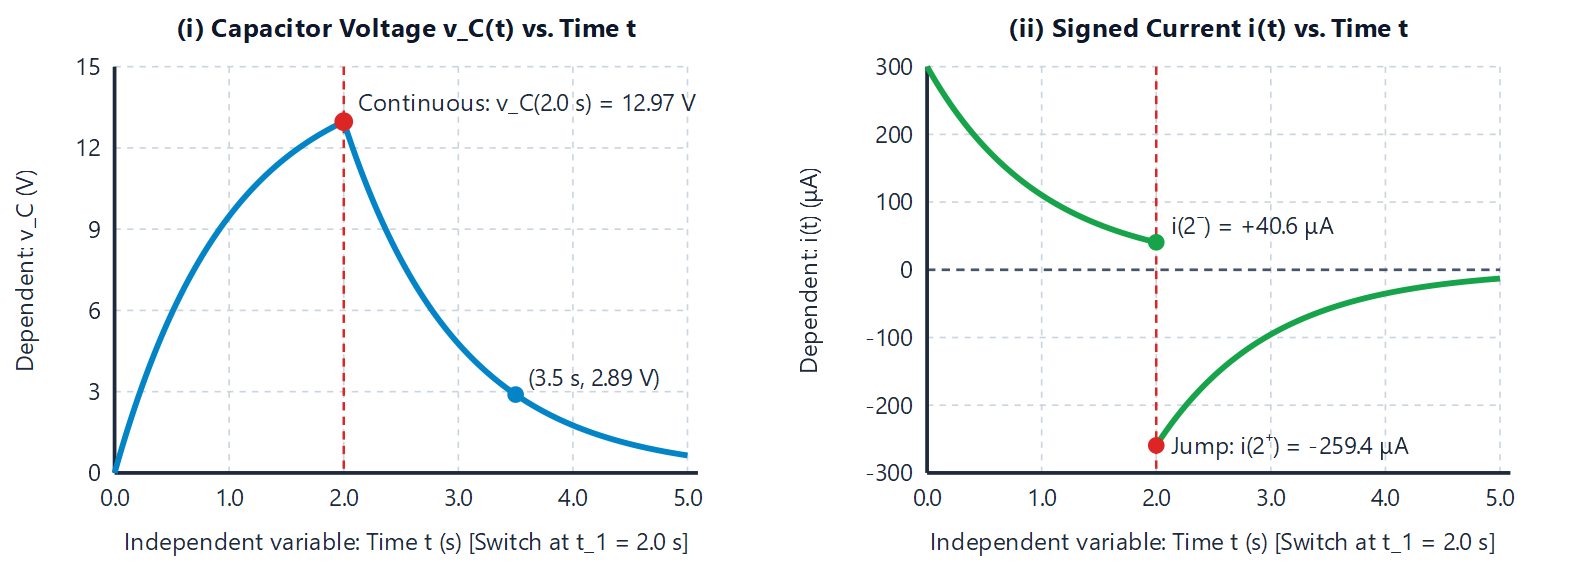
\includegraphics[width=0.82\linewidth]{day1_assets/s3-q4-grid-solved.png}\end{center}

\end{document}
